\chapter{Algoritmo Push and Relabel (Preflow)}

Questa tecnica implementativa si differenzia dagli algoritmi visti fino ad ora in
quanto non utilizza l'idea di \textit{augmenting path}.

\section{Design dell'algoritmo}

La differenza sostanziale è che l'algoritmo Preflow non va ad utilizzare la
funzione \textbf{augment} per cercare di aumentare il flusso su un cammino $u -
	v$, ma cerca di aumentare il flusso arco ad arco.

Solitamente se si usa questo approccio verranno violate le condizioni di
conservazione del flusso, quindi per il corretto funzionamento andremo a
rilassare la condizione di conservazione introducendo un valore di
\textbf{Preflow}.

\begin{myblockquote}
	Un \textit{$s-t$ preflow } è una funzione $f$ che mappa ogni arco $e$ ad un
	numero reale non negativo, $f: E \rightarrow \mathbf{R^+}$.
\end{myblockquote}

Un \textit{preflow} $f$ deve rispettare la capacity condition, ma al posto della
conservetion condition utilizzeremo una condizione meno restrittiva, e dunque
avremo quanto segue:
\begin{enumerate}
	\item \textbf{Capacity}: Per ogni nodo $e \in E$, avremo che $0 \le f(e) \le
		      c_e$
	\item \textbf{Conservation}: Per ogni nodo $v$ al di fuori della source $s$
	      avremo che:
	      $$
		      \sum_{e \text{ into }v}f(e) \ge \sum_{e \text{ out of }v}f(e).
	      $$
\end{enumerate}

Chiameremo la differenza
$$
	e_f(v) = \sum_{e \text{ into }v}f(e) - \sum_{e \text{ out of }v}f(e)
$$
l' \textbf{eccesso} del \textbf{preflow} nel nodo $v$.\\

Si può notare che il preflow di ogni nodo all'infuori di $s$ e $t$ in cui
l'eccesso è 0 può essere considerato a tutti gli effetti come del flow.

\subsection{Preflow e Labelings}
L'algoritmo preflow manterrà un preflow e lo cercherà di convertire in un flow.
Per farlo si basa sull'intuizione fisica che il flusso cerca naturalmente la
strada più in discesa.

L'altezza implicita in questa intuizione sarà rappresentata da dei labels
$h(v)$, che l'algoritmo definirà e manterrà per ogni nodo $v$.

Quindi l'idea è quella di spingere flusso da nodi con label più alto, verso nodi
con label più basso.\\

Ora che abbiamo un idea di come l'algoritmo sfrutta i label possiamo dare una
loro definizione più rigorosa.

\begin{myblockquote}
	Un labeling è una funzione $h: V \rightarrow \mathbf{Z}_{\ge 0}$ che mappa
	nodi a interi non negativi
\end{myblockquote}

Il prossimo passo per creare l'algoritmo è quello di definire un labeling
\textbf{compatibile}, che si avrà quando saranno rispettate le seguenti
condizioni:
\begin{enumerate}
	\item \textbf{Source and Sink condition}: $h(t) = 0$ e $h(s) = n$,
	\item \textbf{Steepness condition}: Per tutti gli archi $(v,w) \in E_f$ nel
	      grafo residuale, avremo che $h(v) \le h(w) + 1$
\end{enumerate}

\begin{figure}[H]
	\centering
	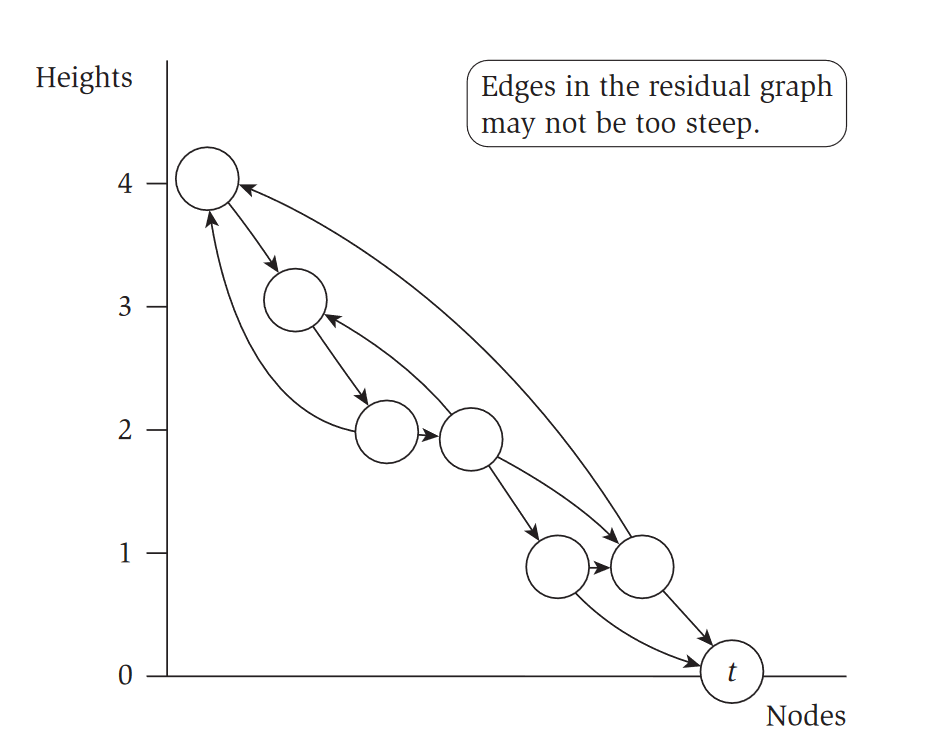
\includegraphics[width = 10 cm]{capitoli/network_flow/imgs/preflow1.png}
	\caption{Grafo residuale con labeling compatibile}
\end{figure}

Se il labeling è compatibile allora avremo la seguente proprietà:
\begin{myblockquote}
	se un \textit{$s-t$ preflow f} è compatibile con un labeling $h$, allora non
	ci sarà nessun cammino nel grafo residuale $G_f$.
\end{myblockquote}

e quindi ne segue:
\begin{myblockquote}
	se un \textit{$s-t$ preflow f} è compatibile con un labeling $h$, allora il
	flusso $f$ è un \textbf{flusso di valore massimo}
\end{myblockquote}

Per iniziare l'algoritmo sarà necessario partire con un labeling compatibile,
quindi è importante definire un'\textbf{inizializzazione}:

\begin{itemize}
	\item $h(v) = 0$ per ogni nodo $v \neq s$,
	\item $h(s) = n$
	\item $f(e) = c_e$ per ogni arco $e = (s,v)$ uscente da $s$
	\item $f(e) = 0$ altrimenti
\end{itemize}

Gli ultimi due punti servono per assicurarsi che non ci siano archi uscenti da
$s$ nel grafo residuale, in quanto il preflow e il labeling iniziali devono
essere compatibili.

\subsection{Pushing e Relabeling}
Andiamo ora ad analizzare gli step dell'algoritmo che trasformano il preflow in
un flow possibile, mantenendo sempre un labeling compatibile.\\

Consideriamo un qualsiasi nodo $v$ con $e_f(v)>0$ (\textit{quindi che ha
	eccesso}). Se esistono degli archi nel grafo residuale che escono da $v$ e vanno
in un altro nodo $w$ che si trova ad altezza inferiore, allora possiamo
modificare $f$ spingendo dell'eccesso da $v$ in $w$.\\

\textbf{Questa si chiama operazione di push}:

\begin{lstlisting}[language=Python, mathescape=true]
push(f , h, v, w)
    Applicable if e_f(v) > 0, h(w) < h(v) and (v, w) $\in$ E_f
    If e = (v, w) is a forward edge then
        let $\delta$ = min(e_f (v), c_e - f(e)) and 
        increase f(e) by $\delta$
    If (v, w) is a backward edge then
        let e = (w, v), $\delta$ = min(e_f(v), f(e)) and
        decrease f(e) by $\delta$
    Return(f, h)
\end{lstlisting}

se non si può spingere dell'eccesso di $v$ lungo uno qualsiasi dei suo archi
uscenti, allora sarà necessario alzare la sua altezza $h(v)$.\\

\textbf{Questa si chiama operazione di Relabel}:
\begin{lstlisting}[language=Python, mathescape=true]
relabel(f , h, v)
    Applicable if e_f(v) > 0, and
        for all edges (v, w) $\in$ E_f we have h(w) $\ge$ h(v)
    Increase h(v) by 1
    Return(f, h)
\end{lstlisting}

Entrambe queste operazioni verranno chiamate in combinazione dell'algoritmo
preflow, che ha il seguente pseudocodice.

\begin{lstlisting}[language=Python, mathescape=true]
Preflow-Push
    Initially h(v) = 0 for all v $\neq$ s and h(s) = n and
    f(e) = c_e for all e = (s, v) and f_(e) = 0 for all other edges
    While there is a node v $\neq$ t with excess e_f(v) > 0
        Let v be a node with excess
        If there is w such that push(f, h, v, w) can be applied then
            push(f, h, v, w)
        Else
            relabel(f , h, v)
    Endwhile
    Return(f)
\end{lstlisting}

\subsection{Analisi dell'Algoritmo}
Ovviamente questa implementazione è solo un idea generale e lascia spazio per
ottimizzazioni.\\

Proviamo ora ad analizzare il \textbf{numero di operazioni} di push e di relabel
che vengono effettuate dal nostro algoritmo per riuscire a stabilirne la
complessità.

Come primo passo definiamo questo semplice fatto:
\begin{myblockquote}
	\begin{minipage}{\textwidth}
		\begin{definition}
			Sia $f$ un preflow, se il nodo $v$ ha eccesso allora esiste un cammino in
			$G_f$ da $v$ alla source $s$
		\end{definition}
	\end{minipage}
\end{myblockquote}

Detto questo possiamo dimostrare che i label non vengono modificati troppe
volte:

\begin{myblockquote}
	Durante l'algoritmo tutti i nodi hanno $h(v) \le 2n-1$.
\end{myblockquote}

\begin{proof}
	Le labels inziali $h(t) = 0$ e $h(s) = n$ non cambiano mai
	durante l'esecuzione dell'algoritmo. Consideriamo altri nodi $v \neq s, t$.
	L'algoritmo cambia la label di $v$ solo quando applica l'oprazione di
	\textbf{relabel}, quindi siano $f$ e $h$ il preflow ed il labeling ritornati
	dalla funzione \textbf{relabel}($f , h, v$). Dalla definizione precedente a
	questa esiste un cammino P nel grafo residuale $G_f$ da $v$ a $s$. Sia $|P|$ il
	numero di archi in $P$, e si noti che $|P| \leq n - 1$. La steepness condition
	implica che l'altezza dei nodi può diminuire di al massimo 1 lungo ogni arco in
	$P$, e che $h(v) - h(s) \leq |P|$, il che prova l'affermazione di partenza.
\end{proof}

Dato che i label incrementano in modo \textbf{monotono} durante l'esecuzione
dell'algoritmo, questa cosa ci implica un limite immediato al \textbf{numero di
	operazioni di relabeling}:

\begin{myblockquote}
	Durante l'algoritmo ogni nodo subisce relabeling al massimo $2n-1$ volte, e
	il numero totale di operazioni di releabeling serà minore di $2n^2$
\end{myblockquote}

Ora cerchiamo un \textbf{bound} per le operazioni di push, per farlo
distingueremo \textbf{2 tipi di operazioni push}.
\begin{itemize}
	\item un $push(f, h, v, w)$ è \textbf{saturante} se o $e = (v, w)$ è un arco
	      forward in $E_f$ e $\delta = c_e - f(e)$, oppure $(v,w)$ è un arco backward
	      con $e = (w,v)$ e $\delta = f(e)$(\textit{in altre parole se dopo il push
		      l'arco $(v,w)$ non è più nel grafo residuale, allora il push è saturante}).
	\item il push è \textbf{non saturante} in tutti gli altri casi
\end{itemize}

\begin{myblockquote}
	Il numero massimo di operazioni \textbf{push saturanti} è al massimo $2nm$
\end{myblockquote}

\begin{proof}
	Consideriamo un arco $(v, w)$ nel grafo residuale. Dopo un push saturante
	\textbf{push}($f, h, v, w$), abbiamo che $h(v) = h(w) + 1$, e che l'arco $(v,
		w)$ non è più presente nel grafo residuale $G_f$. Prima di poter fare
	un'operazione di push in quest'arco dobbiamo prima fare un'operazione di push da
	$w$ a $v$ per far apparire l'arco $(v, w)$ nel grafo residuale. Però, per poter
	fare un'operazione di push da $w$ a $v$, la label di $w$ deve aumentare di
	almeno 2 (così che $w$ sia al disopra di $v$). La label di $w$ può aumentare di
	2 al massimo $n - 1$ volte, perciò un push saturante da $v$ a $w$ può avvenire
	al massimo $n$ volte. Ogni arco $e \in E$ può dar luogo a due archi nel grafo
	residuale, quindi in generale possiamo avere al massimo $2nm$ push saturanti.
\end{proof}


Per quanto riguarda i push non saturanti, provare un loro upper-bound è la parte
più difficile di questa analisi ma anche la più importante perchè ci fornisce un
\textbf{bottleneck} per il running time teorico.

\begin{myblockquote}
	Il numero di operazioni di \textbf{push non saturanti} è al più $2n^2m$
\end{myblockquote}

\begin{proof}
	Per questa dimostrazione utilizzaremo una
	\textbf{funzione potenziale}, definita come segue:
	$$
		\Phi(f, h) = \sum_{v:e_f(v)>0}h(v)
	$$
	Sarà la somma delle altezze dei noti con eccesso positivo (è chiamata
	\textit{potenziale}, perchè assomiglia all'energia potenziale dei nodi con
	eccesso positivo).\\

	Nella configurazione iniziale $\Phi(f, h) = 0$, successivamente rimarrà sempre
	non negativa durante tutta l'esecuzione dell'algoritmo.

	Per ogni operazionie di push non saturante $push(f, h, v, w)$, $\Phi(f, h)$
	viene decrementata di almeno 1, in quanto dopo il push il nodo $v$ non avraà più
	eccesso, e $w$, l'unico nodo che ottiene nuovo eccesso da $v$ si trova di 1
	sotto a $v$.

	Tuttavia, ogni \texttt{push saturante} e ogni \texttt{relabel} possono
	incrementere $\Phi(f, h)$. Una \texttt{relabel} incremente $\Phi(f, h)$ di
	esattamente 1, e dato che ci stanno al massimo $2n^2$ \texttt{relabel}
	l'incremente massimo di $\Phi(f, h)$ sarà di $2n^2$.

	Un \texttt{push}$(f, h, v, w)$ saturante non cambia le label, ma può comunque
	aumentare $\Phi(f, h)$ a causa del potenziale incrementeo di eccesso del nodo
	$w$.

	Questp può incrementare $\Phi(f, h)$ dell'altezza di $w$, che è al massimo
	$2n-1$, e visto che ci sono al massimo $2nm$ \texttt{push} saturanti,
	l'incremente totale  in $\Phi(f, h)$ causato dalle operazioni di \texttt{push} è
	al massimo $2mn(2n-1)$.
\end{proof}

Quindi tra \texttt{push} saturanti e \texttt{relabel} il numero massimo di
incrementi sarà $2mn^2$, da qui ne deriva che, considerando che $\Phi$ rimane
non negativa, e viene decrementata di almeno 1 per ogni operazione di
\texttt{push} non saturante, avremo al massimo $4mn^2$ operazioni di
\texttt{push} non saturanti.\\

Con determinati criteri è possibile ridurre il numero di push non saturanti:

\begin{myblockquote}
	Se ad ogni step scegliamo il nodo con eccesso ad altezza massima, il numero
	di \textbf{push non saturanti} sarà al massimo $4n^3$
\end{myblockquote}